\section{Discussion}

This section will discuss the acoustic suitability of the new office development.
This will first be done in terms of ductwork noise transmission between the plant room and conference room.
Then it will be done in terms of sound transmission between the conference room and the adjacent single office, as there is concern that the speech may be audible in the office.



\subsection{Ductwork noise transmission} \label{sec:disc_BN}

%\textbf{From Q1 and Q4.3:}
%It is interesting to note that the SPLs at 63~Hz and 125~Hz are low relative to the other SPLs.
%This is largely because of the high end reflection losses at low frequencies.

The SPL in the conference room due to fan noise transmitted through the ductwork, L\textsubscript{p\textsubscript{1}}, has led to a slightly high noise rating of NR~50.
This could cause some intelligibility issues during conversations held in the conference room.
As the single office's reverberation time and ductwork attenuations are similar to the conference room's, the single office has a similar SPL due to fan noise (see Figure~\ref{fig:Lp1+2}) which has led to the same noise rating of NR~50.
Occupants in the office might therefore experience the same intelligibility difficulties.

To reduce the rooms' noise ratings to the recommended range of NR~25-45, the fan noise needs to be controlled.
It is of interest to apply the `source - path - receiver' approach to prevent high noise ratings in further rooms served by the same ductwork.

Firstly, noise should be controlled at the source.
In this case, the supply and extract fans could be replaced with quieter fans, if possible.

Secondly, noise should be controlled along the path.
The ductwork is rectangular which already provides higher attenuation compared to circular ducts.
Control measures that could be applied in this scenario include:
\begin{itemize}
	\item Replacing the sound attenuator with one that provides higher levels of attenuation.
	\item Increasing the external lagging on the ductwork.
	\item Reducing air turbulence through the use of deflectors at branches and carefully shaped grilles and diffusers at duct terminations.
\end{itemize}

Lastly, noise should be controlled at the receiver.
If the rooms' sizes are assumed to be unchangeable, this can be done by decreasing their reverberation times (see Equation~\ref{eq:SPL}; a smaller T leads to a smaller L\textsubscript{p}).
The reverberation times can be decreased by increasing the absorption of the rooms' existing materials or by adding furnishings and people.
Increasing the absorption of the existing materials might not greatly decrease the reverberation times, nor might it be desirable due to the already slightly low reverberation times of the rooms (see Section~\ref{sec:Q2}).

On the contrary, it might be preferable to increase the rooms' reverberation times to be within the recommended range for speech (i.e. between 0.5~s and 1.0~s).
This can be done by increasing the rooms' volumes and/ or by decreasing the rooms' absorptions.
For example, both of these objectives can be achieved by removing the suspended ceiling or reducing the depth of its airspace.

To conclude on the ductwork noise transmission, the proposed design is not ideal.
It is recommended that the fan noise is controlled at the source and/ or along the path to bring the rooms' noise ratings down to NR~25-45.
And, on a side note, it is recommended that the rooms' reverberation times are increased to suit rooms used for speech, i.e. between 0.5~s and 1.0~s.


%The curves for the fan noise transmitted through the ductwork, L\textsubscript{p\textsubscript{1}} and L\textsubscript{p\textsubscript{2}}, in Figure~\ref{fig:Lp1+2} are similar because the reverberation times of the rooms and attenuations are similar.
%However, the path from the fan to the single office consistently has more attenuation across all frequencies than the path to the conference room because of the longer horizontal ductwork.
%This is why the L\textsubscript{p\textsubscript{2}} curve is generally below the L\textsubscript{p\textsubscript{1}} curve, with a maximum difference of about 8~dB at 63~Hz.
%L\textsubscript{p\textsubscript{2}} is only slightly higher than L\textsubscript{p\textsubscript{1}} above 1~kHz; this is because the single office is smaller than the conference room.

%These similar SPLs due to fan noise lead to very similar NR ratings.
%Since L\textsubscript{p\textsubscript{1}} and L\textsubscript{p\textsubscript{2}} both peak at about 45~dB at 4~kHz, which happens to lie on the NR~50 curve of the NR chart, the conference room and single office both have noise ratings of NR~50.

%\textbf{From Q2:}
%According to Table~2.5 in the course notes \citep{unit2}, the recommended NR for an office ranges between 25 and 45.
%The NR~50 noise rating for the conference room and single office can therefore be perceived as a bit high.

% REDUCE NR
%To reduce the rooms' noise ratings to a more comfortable level, i.e. between 25 and 45, the SPLs due to fan noise must be reduced.
%Therefore, if the addition of furnishings and people do not sufficiently decrease the noise ratings, using a more powerful sound attenuator might be necessary.



\subsection{Sound transmission between the conference room and single office}

Since the speech in the conference room has been found to be slightly audible in the single office, the design target has not been met.
If the concern had only to do with speech being intelligible in the office, this design solution would work.
But since audibility was the concern, this section will discuss how to remove audibility of speech in the office.

For speech in the office to be inaudible, $D_{nT,w} + NR$ should be greater than 80~dB.
Considering the recommendation in Section~\ref{sec:disc_BN} to decrease the noise ratings of the rooms, D\textsubscript{nT,w} needs to be further increased to overcome the 80~dB threshold.
In its current state, the D\textsubscript{nT,w} through the partition exceeds this threshold, even if the office's NR rating were as low as NR~25.
Hence, more effort will be needed to increase the D\textsubscript{nT,w} through the ductwork, which fails to exceed this threshold.

Increasing D\textsubscript{nT,w} means increasing D\textsubscript{nT}.
To increase D\textsubscript{nT} (see Equation~\ref{eq:DnT}), one can increase L\textsubscript{p\textsubscript{male\textsubscript{1}}} or T\textsubscript{2}, or one can decrease the SPL in the office (whether this is L\textsubscript{p\textsubscript{male\textsubscript{2}ducts}}, L\textsubscript{p\textsubscript{male\textsubscript{2}partition}} or L\textsubscript{p\textsubscript{male\textsubscript{2}}}).
Assuming T\textsubscript{2} increases as per the recommendation in Section~\ref{sec:disc_BN} and L\textsubscript{p\textsubscript{male\textsubscript{1}}} is constant, the only variable we can change is the SPL in the office.

To decrease L\textsubscript{p\textsubscript{male\textsubscript{2}ducts}}, the attenuation along the ductwork between the conference room and single office needs to increase (see Equation~\ref{eq:power_out}).
Again, the ductwork is rectangular which already provides higher attenuation compared to circular ducts.
Assuming the duct sizes will not change, the following measures can be applied:
\begin{itemize}
	\item Add a sound attenuator along the ductwork between the conference room and single office (the closer to the conference room, the better).
	\item Increase the external lagging on the ductwork.
	\item Reduce air turbulence through the use of deflectors at branches and carefully shaped grilles and diffusers at duct terminations. 
\end{itemize}

To decrease L\textsubscript{p\textsubscript{male\textsubscript{2}partition}} (see Equation~\ref{eq:SRI_rearranged}), one can decrease L\textsubscript{p\textsubscript{male\textsubscript{1}}} or S\textsubscript{partition}, or one can increase R or A\textsubscript{2}.
As discussed in Section~\ref{sec:disc_BN}, increasing A\textsubscript{2} would be undesirable as it would further decrease the already low reverberation time in the office, T\textsubscript{2}.
Assuming L\textsubscript{p\textsubscript{male\textsubscript{1}}} and S\textsubscript{partition} to be constant, the only variable that can be changed is the SRI of the partition, R.
As R is independent of the rooms and the partition size, it can only be changed by altering other properties of the wall.
As the partition is a membrane absorber, changing its panel mass or the depth of the air space can change its frequency of maximum absorption.
Ensuring the partition wall has mineral wool in its cavity will significantly improve the wall's insulation properties at mid and high frequencies (as is the case in the design proposal).
However, increasing the discontinuity between the partition's two leaves (e.g. by detaching the wall ties) can further improve the wall's sound reduction properties, by up to 10~dB.

To conclude on the sound transmission between the conference room and single office, the proposed design solution does not meet the design target.
Considering that single office's noise rating is recommended to decrease, the D\textsubscript{nT,w} between the rooms needs to further increase to exceed the 80~dB threshold for inaudibility.
It is recommended that the attenuation between the conference room and single office is increased.
If necessary, the partition wall can also be replaced with one that has a higher SRI.

It should be stressed that, combined, the ductwork and partition are only as effective at reducing the voice transmission as they are least effective individually (see Figure~\ref{fig:DnT}).
This is why the pink D\textsubscript{nT} curve for both the ductwork and partition follows the troughs of the separate D\textsubscript{nT} curves for the ductwork (orange) and partition (green).
In other words, even though the ductwork is most effective at reducing the sound level at lower frequencies, the partition wall still lets sound through at these frequencies (and vice-versa at higher frequencies).
Therefore, it is necessary for the D\textsubscript{nT,w} through the ductwork plus the office's noise rating to exceed the 80~dB threshold.


%\textbf{From Q3:} Comment on Figure~\ref{fig:Lpmale}:
%\begin{itemize}
%	\item The ductwork attenuated mostly on the lower end of the spectrum (up to 58~dB); this is mostly due to high end reflection losses (c.f. Question 1)
	
%	\item The partition is more effective at reducing sound at the higher end of the frequency spectrum (up to 78~dB). This is because L\textsubscript{p\textsubscript{male\textsubscript{2}partition}} varies with R and A\textsubscript{2}, which are both more effective sound level reducers at the higher end of the frequency spectrum.
%	\begin{itemize}
%		\item The SRI of the partition, R, is independent of the wall or room properties.
%		The effectiveness of the partition at reducing sound generally increases with frequency (see R in graph, where it peaks with 64~dB at 2~kHz).
		
%		\item A\textsubscript{2} is the sum of surface absorptions in the single office.
%		The A\textsubscript{2} curve in the graph resembles the curve of a combined membrane and porous absorber with two peaks (19.7~m\textsuperscript{2} at 125~Hz and 27~m\textsuperscript{2} at 4~kHz).
%		The single office thus has slightly more absorption on the higher end of the frequency spectrum.
%	\end{itemize}

%	\item The sum of the SPLs in the single office basically consists of the peaks of L\textsubscript{p\textsubscript{male\textsubscript{2}ducts}} and L\textsubscript{p\textsubscript{male\textsubscript{2}partition}}.
%\end{itemize}

%\begin{figure}[htbp]
	\centering
	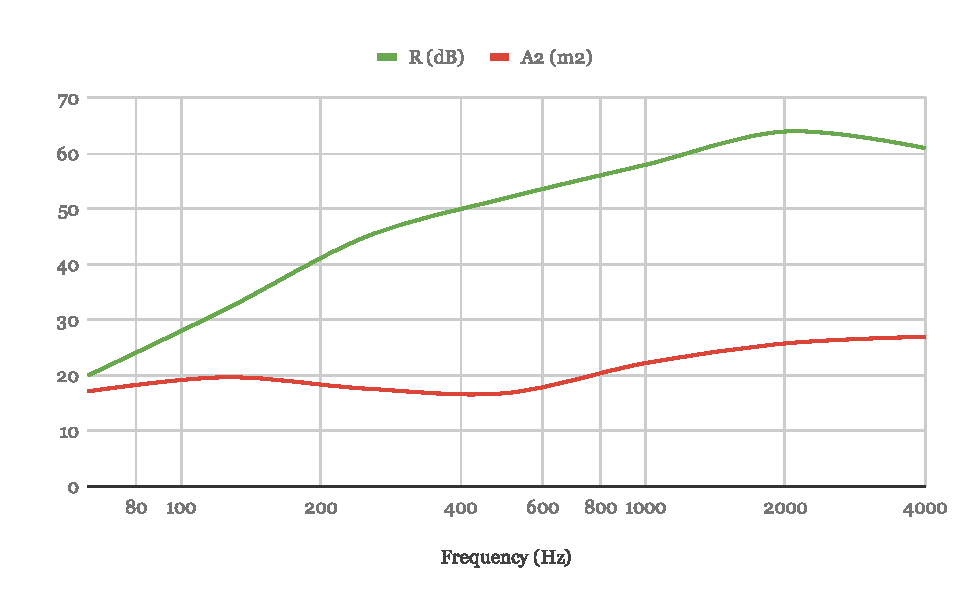
\includegraphics[width=\textwidth]{figures/R+A2.eps}
	\rule{\textwidth}{0.5pt} % use line???
	\caption{The partition's SRI, R, and the single office's total absorption, A\textsubscript{2}.}
	\label{fig:R+A2}
\end{figure}

%\textbf{Q4:}
%\begin{itemize}
%	\item The D\textsubscript{nT} curves in Figure~\ref{fig:DnT} resemble a mirror reflection of the SPL curves of the male voice in the single office in Figure~\ref{fig:Lpmale}.
%	This makes sense as D\textsubscript{nT} is approximately equal to L\textsubscript{p\textsubscript{male\textsubscript{1}}} minus L\textsubscript{p\textsubscript{male\textsubscript{2}\ldots}}.
%	(The standardisation provided by the addition of $10 log \frac{T_2}{0.5}$ makes D\textsubscript{nT} vary from the simple level difference, $D = L_1 - L_2$, by no more than 3~dB.)
%	So much like was said before:
%	\begin{itemize}
%		\item The ductwork is least effective at reducing the sound level at the higher end of the frequency spectrum.
%		\item The partition is least effective at the lower end of the spectrum.
%		\item Combined, the ductwork and partition are only as effective at reducing the sound level as they are least effective individually.
%		This is why the pink D\textsubscript{nT} curve for both the ductwork and partition follows the troughs of the separate D\textsubscript{nT} curves for the ductwork (orange) and partition (green).
%		In other words, even though the ductwork is most effective at reducing the sound level at lower frequencies, the partition wall still lets sound through at these frequencies (and vice-versa at higher frequencies).
%	\end{itemize}
	
%	\item D\textsubscript{nT,w} is the weighted standardised level difference, i.e. a single number which corresponds to subjective perception according to a rating method (ISO 717).
%	Similarly to the previous point, combined, the ductwork and partition are only as effective at reducing the sound level as they are least effective individually.
%	Hence,the combined D\textsubscript{nT,w} value is equal to the D\textsubscript{nT,w} for the ductwork (29~dB) which is less than the D\textsubscript{nT,w} for the partition (56~dB).
	
%	\item The client might prefer to not hear anything at all from the conference room.
%	How to increase DnT?
%	Do we want to reduce NR?
%	Do we want to increase T?
%\end{itemize}

%Suggestions/ improvements?
%\begin{itemize}
%	\item The carpet's mid-frequency absorption properties can be improved by increasing its thickness
%	\item Double glazed windows: Changing the panel mass or the depth of the air space can change the frequency of maximum absorption
%	\item Suspended ceiling?
%	\item Partition?
%\end{itemize}

%\textbf{From Background:}
%\begin{itemize}
%	\item It is likely that the thin carpet on concrete and 10~mm double glazed windows will be the cheapest among their counterparts, since they do not absorb sound as well.
%	It will be interesting to find out whether the cheapest and ``worst performing" materials in the proposed design solution will meet the privacy requirements of the conference room.
%	If they do not, one can then consider using more absorptive (and possibly more expensive) materials.
	
%	\item The arithmetic averages of the reverberation times in the conference room and single office are respectively 0.41~s and 0.40~s.
%	Considering that the typical reverberation time of rooms used for speech is between 0.5~s and 1.0~s, these results are a bit low.
%	This might be perceived as uncomfortable by the occupants, especially when they and the furnishings will further add absorption and shorten the reverberation times in the rooms.
%\end{itemize}